%#! platex thesis.tex

%======================================================================
\chapter{はじめに}
\label{cha:intro}

%----------------------------------------------------------------------
\section{タイプセットの仕方}

TeXがインストールされていれば,
\begin{quote}
 \texttt{\$ make}
\end{quote}
を実行すればPDFファイルが生成される.
なお,\textbf{デフォルトの\texttt{Makefile}は\texttt{thesis.tex}の変更し
か参照しない}ため,必要であれば43行目にtexファイル名を追加する.
\texttt{make clean}するとPDFファイル以外で生成された中間ファイルの一部が
削除される.
また,\texttt{make cleanup}するとタイプセットに必要無いファイルはPDFファ
イルも含めて全て削除される.
Google Driveなどに登録する際は\texttt{make clean}してから登録すると良い.

\texttt{make}コマンドをインストールしていない場合は\texttt{platex}と
\texttt{pbibtex}(または\texttt{jbibtex})を適切な回数
(\texttt{platex}→\texttt{pbibtex}→\texttt{platex} 2回)実行し,
\texttt{.dvi}ファイルを生成する.
\begin{quote}
 \texttt{\$ platex thesis.tex}

 \texttt{\$ pbibtex thesis}

 \texttt{\$ platex thesis.tex}

 \texttt{\$ platex thesis.tex}
\end{quote}

その後\texttt{dvipdfmx}を使ってPDFを生成する.
\begin{quote}
 \texttt{\$ dvipdfmx thesis.dvi}
\end{quote}

なお,\texttt{make}では\texttt{pbibtex}も自動で実行するので,参考文献を
手で修正する場合は\texttt{.bbl}ファイルを\texttt{ref.tex}などの名前に変
更し,\texttt{Makefile}の
\begin{quote}
 \texttt{BIB = echo}
\end{quote}
を有効化すること.

\texttt{listings}パッケージを利用するとソースコード等の掲載が楽になる.
Macなどではデフォルトでインストールされているかと思うが,もしない場合は
\url{http://www.akita-nct.ac.jp/yamamoto/comp/latex/make_doc/source/source.html#listings}
あたりを参考にしてインストールする.
使い方は
\url{http://www.biwako.shiga-u.ac.jp/sensei/kumazawa/tex/listings.html}
あたりが参考になる.

なお,\texttt{make clean}すると中間ファイルを削除できる.
\texttt{make cleanup}とした場合には生成されたPDFファイルも削除される.

%----------------------------------------------------------------------
\section{このテンプレートの構成}

\begin{table}[bt]
 \centering
 \caption{テンプレートのファイル構成}
 \label{tab:files}
 \begin{tabular}{ll}\Hline
  各種\texttt{tex}ファイル & \texttt{thesis.tex}\\
  & \texttt{intro.tex}\\
  & \texttt{conclu.tex}\\
  & \texttt{ack.tex}\\
  & \texttt{public.tex}\\ \hline
  resume用ファイル & \texttt{resume.tex}\\
  & \texttt{resume.sty}\\ \hline
  修論・卒論スタイルファイル & \texttt{jgraduate.sty}\\ \hline
  信学会BiBTeXスタイルファイル & \texttt{sieicej.bst}\\ \hline
  ビルド設定 & \texttt{Makefile}\\ \hline
  サンプルbibファイル & \texttt{bib/}\\ \Hline
 \end{tabular}
\end{table}

\tablename~\ref{tab:files}に,このテンプレートに含まれているファイルを示
す.

章を追加する場合はファイルを追加する.
章ファイルの書き方は\texttt{conclu.tex}をマネすれば良い.
章ファイルを作成したら,\texttt{thesis.tex}に\texttt{\yen include}文を追
加する.

%----------------------------------------------------------------------
\section{基本情報の書き換え}

以下のファイルには名前や所属などの基本情報が書かれているため,全て書き換
えること.

\begin{enumerate}
 \item \texttt{thesis.tex}

       \texttt{pdfauthor},
       \texttt{pdftitle},
       \texttt{\yen title},
       \texttt{\yen author},
       \texttt{\yen university},
       \texttt{\yen department},
       \texttt{\yen major},
       \texttt{\yen date}
 \item \texttt{resume.tex}

       \texttt{\yen title},
       \texttt{\yen author},
       \texttt{\yen professor},
       \texttt{\yen date},
       \texttt{\yen time},
       \texttt{\yen location}
\end{enumerate}

%----------------------------------------------------------------------
\section{論文記述に関する基本的なルール}

\begin{enumerate}
 \item 主語を省略しないこと.
       省略していいのは2つの文が連続で同じ主語のときだけ.
       3つの文が連続して同じ主語になるのは好ましくないので,そのような場
       合には文を書き換えること.
 \item 1段落(1 paragraph)には1つの話題(topic)のみを記述する.
 \item 大事なことは最初に書く.
       例外は論文の一番最初の段落.
 \item 主語と述語を対応させる.
 \item 原則として1つの文は全角36文字折り返しで3行以内にする.
\end{enumerate}

%----------------------------------------------------------------------
\section{印刷に際する注意}

マージン(余白)が少ないと事務に提出する際に突き返される.
2015年度の規定では,上下の余白は30\,mm以上,左右の余白は25\,mm以上となっ
ている.

デフォルト設定では倍率100\,\%で印刷して大丈夫なようにしてあるが,環境に
よっては余白が小さくなるため必要に応じて\texttt{thesis.tex}内の
\texttt{geometry}パッケージのオプションを変更すること.

%----------------------------------------------------------------------
\section{Tips}

%--------------------------------------------------
\subsection{全般}

\begin{itemize}
 \item 情報系の論文は句読点として「,」「.」(全角)を用い,「〜だ」「〜
       である」調で記述する.
 \item 日本語本文中に括弧を使う場合は(このようにして)全角を使うこと.
       流儀にもよるが,基本的には中身が英語であっても全角を用いる(like
       this).
 \item 「1つ」などと数字を使った表記をする場合は半角の数字を使うこと.
 \item マイナスの数字で「-」と書くとハイフンになってしまうので,$-52$の
       ように数式モードを使うこと.
 \item \textbf{全角スペースは絶対に使用しない}こと!
 \item \texttt{\~}(半角チルダ)は改行されないスペースである.
       図表番号を記述する際などに使用する.
 \item コマンドなどは\texttt{make}などとして記述する.
 \item 単位や規格番号の前には\texttt{\yen ,}を入れると少しスペースが空い
       て見やすくなる.10\,mやIEEE\,802.15.4など.
 \item 図に英語を入れると福田先生に日本語にしろと言われるため,図は日本
       語で作成する.
       ただし,一般の論文では図は英語で書くことが望ましいため,日本語と
       英語の両方を作成しておく.
       \textbf{図の元ファイル(pptなど)も必ず残しておく}こと.
 \item 実験結果のグラフなどは,どのデータをどうやって描いたかが分かるよ
       うな記録を必ず残す.
       結果が間違っていたときに変更できないと捏造になるので注意すること.
 \item 英文における「.」(ピリオド)の使い方に注意.
       TeXでは
       \begin{enumerate}
        \item 大文字の後ろのピリオドでは終止符ではない.
        \item それ以外のピリオドは終止符.
       \end{enumerate}
       と判断されるため,「\texttt{GPS.}」のような場合にはピリオドが終止
       符でないと判断される.
       この場合は「\texttt{GPS\yen@.}」と書くこと.
       括弧は無視されるので,「\texttt{(GPS).}」のような場合も
       「\texttt{(GPS)\yen@.}」と書くこと.
       逆に,\texttt{Fig. 1}のような場合は「\texttt{Fig.\yen\ 1}」
       や「\texttt{Fig.\~{}1}」などと明示的にスペースを入れることで終止
       符でないことを示す.
\end{itemize}

%--------------------------------------------------
\subsection{図}

\begin{figure}[bt]
 \centering
 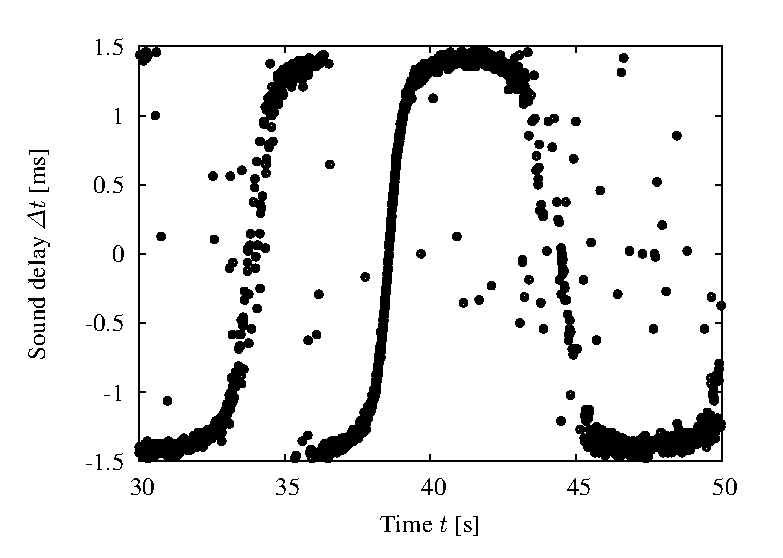
\includegraphics[width=\figurewidth]{img/test.eps}
 \caption{ダミーの図}
 \label{fig:test}
\end{figure}

図や表を入れる際の\texttt{figure},\texttt{table}環境のオプションでは
\texttt{[h]}は指定せず,\texttt{[bt]},\texttt{[btp]}などとする.

図を真ん中に表示させるには,\figurename~\ref{fig:test}のように
\texttt{\yen centering}を使う.
\texttt{center}環境を使うとムダなスペースが入ってしまう.
また,図や\texttt{section}を参照する場合は\texttt{\yen label}と
\texttt{\yen ref}を使う.

\begin{figure}[bt]
 \centering
 \begin{minipage}[b]{0.49\hsize}
  \centering
  \fbox{\rule{0pt}{2cm}\rule{0.4\figurewidth}{0pt}}\\
  (a)~ダミーの図1-1
 \end{minipage}
 \hfill
 \begin{minipage}[b]{0.49\hsize}
  \centering
  \fbox{\rule{0pt}{2cm}\rule{0.4\figurewidth}{0pt}}\\
  (b)~ダミーの図1-2
 \end{minipage}
 \caption{ダミーの図(横並べバージョン)}
 \label{fig_intro:dummy_fig1}
\end{figure}

\begin{figure}[bt]
 \centering
 \fbox{\rule{0.8\hsize}{0pt}\rule{0pt}{2cm}}\\
 (a)~ダミーの図2-1
 \vspace{\figuresep}

 \fbox{\rule{0.8\hsize}{0pt}\rule{0pt}{2cm}}\\
 (b)~ダミーの図2-2
 \caption{ダミーの図(縦積みバージョン)}
 \label{fig_intro:dummy_fig2}
\end{figure}

図を並べる時は\figurename~\ref{fig_intro:dummy_fig1}や
\figurename~\ref{fig_intro:dummy_fig2}のように書く.

%--------------------------------------------------
\subsection{表}

表の書き方は\tablename~\ref{tab:files}を参照のこと.
表に縦線を入れるとダサい感じになる.
区切りに使用するための太線として\texttt{\yen Hline}を用意しているので適
宜利用する.

%--------------------------------------------------
\subsection{リスト}

番号なしのリストは\texttt{itemize}環境を使う.
\begin{itemize}
 \item テスト1
 \item テスト2

       長い場合には段落を変えることもできるが,字下げはデフォルトでは無
       効になっている.
 \item テスト3
\end{itemize}

番号付きのリストは\texttt{enumerate}環境を使う.
\begin{enumerate}
 \item テスト1
 \item テスト2
\end{enumerate}

\texttt{enumerate}パッケージを使えば,番号付きリストにラベルを付けること
もできる.
\begin{enumerate}[(第1段階)]
 \item テスト段階
 \item テスト段階
\end{enumerate}

%--------------------------------------------------
\subsection{数式}

インラインの数式は$y=x^2+x+2$のように\texttt{\$}で囲うことで記述できる.
1行を使う数式は\texttt{equation}環境を使う.
\begin{equation}
 f(x) = \int_0^{2\pi}\frac{\sin x}{x}\,dx
  \label{eq:test_eq}
\end{equation}
数式を参照する場合は,式~(\ref{eq:test_eq})のように\texttt{\yen label},
\texttt{\yen ref}を用いる.

数式番号を付けたくない場合は環境名に\texttt{*}を付ける.
\begin{equation*}
 f(x) = \int_0^{2\pi}\frac{\sin x}{x}\,dx
\end{equation*}


複数行の数式は\texttt{align}環境を使用する.
\texttt{\&}は位置を揃えるためのマークであり,出力はされない.
数式番号を出力したくない行には\texttt{\yen nonumber}を付ける.
\begin{align}
 f(x) &= \int_0^{2\pi}\frac{\sin x}{x}\,dx \nonumber\\
 g(x) &= \int_0^{2\pi}\frac{\cos x}{x}\,dx
\end{align}

括弧を使う場合は大きさが自動的に変わるように\texttt{\yen left}などと組み
合わせて使用する.
\begin{align*}
 S &= \sum_k \delta_{ij}[k] \\
 U &= \sum_k \left( \zeta[k] + 3\sum_{l=0}^k \delta_{ij}[l] \right)
\end{align*}

数式中で複数文字から成る変数を表現する際は,ときと場合によってスペースが
広がりすぎるのを防ぐため\texttt{\yen mathrm}や\texttt{\yen mathit}でまと
める.

\begin{equation*}
 \left\{
 \begin{array}{rcl}
  P_{t1} - L_\mathit{loss} &=& \mathrm{RSS}_1\\
  P_{t2} - L_\mathit{loss} &=& \mathrm{RSS}_2\\
  &\vdots&
 \end{array}
 \right.
\end{equation*}

%--------------------------------------------------
\subsection{引用}

\texttt{.bib}ファイルを作成し,本文中で\texttt{\yen cite}を使って参照す
る~\cite{wu13:will_pds}.
その上で\texttt{pbibtex}または\texttt{jbibtex}を使って\texttt{.bbl}ファ
イルを生成する.
一度に複数書くこともでき
る~\cite{scholten08:cmc_psp,nakauchi05:intelli_kitchen%
,yang12:locate_finger}.


% 以下はRefTeX用
%%% Local Variables:
%%% mode: yatex
%%% TeX-master: "thesis"
%%% End: